\documentclass[b5paper,11pt]{article}
\bibliographystyle{plain}

\usepackage{geometry}
\usepackage{amssymb,amsthm,bm,mathrsfs,mathtools}
\usepackage[usenames]{xcolor}
\usepackage{hyperref}
\usepackage{graphicx}
\graphicspath{{../"img/"}{../"figures/"}}

\usepackage{mycommands}
\newcommand{\numcircled}[1]{\raisebox{.5pt}{\textcircled{\raisebox{-.9pt} {#1}}}}
\newcommand{\Dmax}{\trdis_\mathsf{max}}
\newcommand{\InFmax}{\infid_\mathsf{max}}
\newcommand{\Psb}{\mathcal{P}_\mathrm{SB}}
\newcommand{\Odd}{\Omega_{\mathsf{DD}}}
\newcommand{\Opdd}{\Omega_{\mathsf{PDD}}}
\newcommand{\vOpdd}{\vec{\Omega}_{\mathsf{P}}}
\newcommand{\LO}[1]{\operatorname{LO}}
\newcommand{\alphat}{\widetilde{\alpha}}
\newcommand{\betat}{\widetilde{\beta}}

\newcommand{\Ppb}{\mathscr{P}_{\mathrm{0}}}
\newcommand{\Pcp}{\mathscr{P}_{\mathrm{c}}}
\newcommand{\wtP}{\widetilde{P}}
\newcommand{\wtH}{\widetilde{H}}
\newcommand{\wtO}{\widetilde{\Omega}}
\newcommand{\wtU}{\widetilde{U}}

\newcommand{\HB}{H_\mathrm{B}}
\newcommand{\HSB}{H_\mathrm{SB}}

\newcommand{\Heff}{H_\mathrm{eff}}
\newcommand{\HeffB}{H_\mathrm{eff,B}}
\newcommand{\HeffSB}{H_\mathrm{eff,SB}}

\newcommand{\ep}{\Phi_\mathrm{SB}}
\newcommand{\wtep}{\widetilde{\Phi}_\mathrm{SB}}
\newcommand{\epB}{\Phi_\mathrm{B}}
\newcommand{\phiB}{\phi_\mathrm{B}}

\newcommand{\CDDn}{\mathrm{CDD}_n}
\newcommand{\rDD}{\mathrm{DD}}
\newcommand{\rmax}{\mathrm{max}}
\begin{document}
\section{Accuracy threshold for concatenated DD}\label{sec:threshold}
Next, we turn to the situation of CDD. We can certainly discuss the break-even point for a particular $\CDDn$ sequence, treating it simply as a ``flattened" sequence of pulses, and ask when the error phase after $\CDDn$ is smaller than $\phi_\rSB$ as was done for PDD in the previous section. 
However, what is more interesting is the question of the so-called accuracy threshold for CDD.
As described in the Preliminaries section, CDD tries to achieve better and better noise removal by concatenating the same basic DD scheme---PDD for our discussion here---to higher and higher levels. Here, we are interested in understanding how the noise removal improves as the DD scheme scales up. In fault-tolerant quantum computing, there is the concept of a fault tolerance noise threshold, a strength of the noise below which scaling up the QEC code leads to improved protection against noise, and hence more accurate quantum computation. This threshold is referred to as the accuracy threshold. Here, we ask the analogous question of CDD, whether there is a condition on the noise parameter of the problem such that increasing the CDD level always leads to improved noise removal capabilities. An accuracy threshold for CDD exists if the parameters governing the noise of the situation satisfying a condition $\eta<\eta_0$, such that 
\begin{equation}\label{eq:thresCond}
\Phi_{\mathrm{SB},n+1} < \Phi_{\mathrm{SB},n}\qquad\forall n=1,2,\ldots.
\end{equation}

Below, we examine this for both the ideal CDD case where pulses are perfect, and the noisy CDD case where imperfections in the pulses are allowed.

\newpage
%%%%%%%%%
\subsection{Ideal case}
If a noise threshold indeed exist, then ideal case, where the noise is non-existent, would definitely apply. 
We first consider CDD with perfect pulses. Khodjasteh and Lidar propose in their paper to truncate to th second order term
gave in their paper an estimation of the $\CDDn$ generator as:
\begin{align}\label{eq:cdd-generator-est}
\Omega_{(n)} 
\approx {} & \sigma_0 \otimes 4^n B_0 \notag \\
+\ & \sigma_1 \otimes (-\upi)^{n} 2^{n(n+1)} \ad_{B_0}^{n}(B_1)\\ 
+\ & \sigma_2 \otimes (-\upi)^{n} 2^{n^2} \ad_{B_0}^{n-\!1}( \,[B_0,B_2] - \upi \{B_1,B_3\} \,). \notag
\end{align} 
It is shown in the appendix \ref{app:CDD} that the above expression indeed captures the leading order behavior of $\Omega_{(n)}$. Different from the leading order term in the Magnus series, the leading order ``behavior'' is manifested separately for the pure bath part and the interaction part.  As mentioned in the Preliminaries section, $\CDDn$ achieves $n$th-order decoupling.  From the leading order expression, we see it is indeed so as the interaction part is of $(n+1)$th order.
From \Eqref{eq:cdd-generator-est}, we can 
estimate $\Phi_{\mathrm{B},n} \simeq 4^n\phi_\rB$ and derive an upper bound for for the error phase:
\begin{equation}
\Phi_{\mathrm{SB},n} \lesssim \,
2^{(n+1)^2} \phi_\rB^{n}\,\phi_\rSB \,f_n\!\left(\frac{\phi_\rSB}{\phi_\rB}\right),
 % \left\{
 % \begin{aligned}
 % 2^n, && \frac{\phi_\rSB}{\phi_\rB} \le \sqrt{4^n-1}. \\
 % \sqrt{1+\frac{1}{4}\left(\frac{4^n-1}{\phi_\rSB/\phi_\rB}+\phi_\rSB/\phi_\rB\right)^2}, && \frac{\phi_\rSB}{\phi_\rB} > \sqrt{4^n-1}.
 % \end{aligned}
 % \right.
\end{equation}
where we define the piece-wise function:
\begin{equation}
 f_n(x) =\left\{
 \begin{aligned}
 &1, && x \le  \sqrt{4^n-1}, \\
 &\frac{1}{2^n} \sqrt{\left(\frac{4^n-1}{2x}+\frac{x}{2}\right)^2+1}, &&
 x > \sqrt{4^n-1}.
 \end{aligned}
 \right.
\end{equation}

to remind the reader, $\phi_\rB\equiv\phi_\rB(\tau_0)\equiv\tau_0\Vert \HB\Vert$, and $\phi_\rSB\equiv\phi_\rSB(\tau_0)\equiv\tau_0\Vert\HSB\Vert$, noting the dependence of both quantities on $\tau_0$, the time interval between two consecutive pulses in the CDD sequence. \red{(To reconsider: We need both an upper and lower bound for $\Phi_{\mathrm{SB},n}$, which we have from the estimator [Eq.~\eqref{eq:lu}]. For use in Eq.~\eqref{eq:thresCond}, we should have the lower bound on the RHS of that condition, and upper bound expression on the LHS, for a sufficient condition.) } As mentioned in the Preliminaries section, $\CDDn$ achieves $n$th-order decoupling. This can be understood from the error phase expression: $\Phi_{\mathrm{SB},n}$ after $\CDDn$ is of order $\phi^{n+1}$, for $\phi\sim\phi_\rB, \phi_\rSB$. That $\phi_\rB$ enters the error phase should again be of no surprise---as in the PDD case, $\phi_\rB$ determines how quickly the noise seen by the system evolves, and hence affects the efficacy of DD which does a good elimination of the noise only when the noise remains nearly unchanged for the full DD sequence. 

What is perhaps more surprising is the appearance of factors of $2^n$ and $2^{n^2}$ in $\Phi_{\mathrm{SB},n}$, a new feature in the CDD case \red{(Do these factors also appear in the Khodjasteh-Lidar analysis? Please check and put in a sentence about this.)}. For fixed $\tau_0\equiv \tau$ as $n$ increases (e.g., if $\tau$ is the experimental limit for the switch time between consecutive pulses), such factors mean that the error phase eventually increases for large enough $n$: The exponentially decreasing $\phi^n$ factor is eventually overcome by the super-exponentially increasing $2^{n^2}$ factor. This means there is no accuracy threshold, i.e., there is no level of noise that is weak enough such that $\Phi_{\mathrm{SB},n+1}\leq\Phi_{\mathrm{SB},n}$ for all $n$. Instead, there is an maximal useful level of concatenation level, beyond which further concatenation actually increases the noise seen by the system. Fig.~\ref{fig:estimator-size} plots this situation of fixed $\tau_0$, for increasing concatenation level $n$. We observe the initial decrease of $\Phi_{\mathrm{SB},n}$ as $n$ increases, but this turns around eventually. 

\begin{figure}
    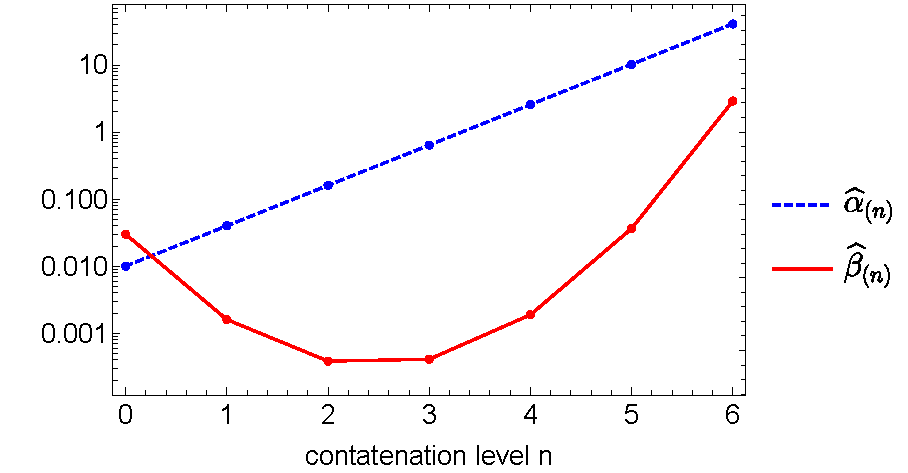
\includegraphics[trim=5mm 0mm 0mm 0mm, clip, width=\columnwidth]{cdd-estimator}
    \caption{The error phase $\phi_{\rSB,n}$ as a function of concatenation level $n$. 
    The thin color lines are obtained from numerically simulating $\CDDn$ with randomly generated bare Hamiltonian operators satisfying $\phi_\rB=1\times10^{-3}$ and $\phi_\rSB=2\times 10^{-3}$. The blue dashed line is our theoretical upper bound. For this configuration, we set the maximal concatenation level at 4.}
    \label{fig:estimator-size}
\end{figure}

\red{(To reconsider with my lower/upper bound comment above.) }
For higher concatenation level to make sense, increasing concatenation level should decrease the error phase. To derive a sufficient condition of it, we examine the recursive relation between concatenation 
levels, which suggests 
\begin{equation}
\begin{aligned}
 B_{n+1,0} &= 4  B_{n,0}\\
 B_{n+1,1} & = -4\upi [B_{n,0}, B_{n,1} ]\\
 B_{n+1,2} & = -2\upi [B_{n,0}, B_{n,1} ]\\
  B_{n+1,3} &=0
\end{aligned}
\end{equation}
For both $B_1$ and $B_2$ to decrease in size, it suffice to require the map 
$-4\upi [B_{n,0},\cdot]$ a contraction map. 
By requiring its norm to be smaller than 1, we obtain the bound for the maximal concatenation level:
\begin{equation}\label{eq:cdd-max-level}
n_{\max}\le \lceil-\log_4(\phi_\rB)-3/2\rceil,
\end{equation}
where $\lceil\cdot\rceil$ is the ceiling operator.

Note that the existence of a maximal useful concatenation level does not technically contradict the statement that 
higher-order decoupling is achieved by higher level CDD. Using decoupling order to quantify the degree of noise removal requires, in the first place, the convergence of the Magnus series, so that the $(n+1)$th- and higher-order terms in the series are a small correction to the first $n$ terms. However, if the DD scheme is designed such that the total time for the sequence grows exponentially with $n$, as is the case for CDD if $\tau_0$ is fixed as $n$ increases, eventually, we exceed the convergence criterion and the decoupling order stops being a reasonable indicator of successful noise removal. 

We can, however, analyze a different situation: to have fixed $\tau_n\equiv T$, so that the CDD sequence takes the same amount of time, regardless of $n$. This requires $\tau_0=\frac{T}{4^n}$ for each $n$, so that the pulses are applied at shorter and shorter time intervals as the concatenation level increases. This can be the practical choice if one is doing computation where computational gates, which can only be applied at the end of a complete DD sequence in order to not interfere with the noise averaging process, have to be applied at a particular clock rate. Increasing $n$ to increase the noise removal capabilities must not increase the total time taken for the DD sequence. This requires, of course, the ability to do faster and faster pulse switching.

In this case, it is more illuminating to make use of $\tau_0\Vert \HB\Vert$ and $\tau_0\Vert\HSB\Vert$, in place of $\phi_\rB$ and $\phi_\rSB$, in our estimate of the CDD error phases, so that that the $n$ dependence in $\tau_0$ is explicit. \red{(I suggest we analyze this case as well, to see if an accuracy threshold exists. Jiaan - could you take a quick look at this?)}
Eventually, of course, this becomes limited by the technological---not fundamental---constraint of how fast we can switch between pulses, and thus how short $\tau_0$ can be in an experiment.


%%%%%%%%%
\subsection{Noisy pulses}
\red{(To add.)}
This has significant implication for the concatenate DD scheme as well, 
as the first order coupling would persist throughout all concatenation levels. 
\appendix
%%%%%%%%%%%%%%%%%%%%%%%%%%%%%
%%%%%%%%%%%%%%%%%%%%%%%%%%%%%
\section{Analyzing $\CDDn$}\label{app:CDD}

It was suggested by the authors of CDD that the decoupling order for $\mathrm{CDD}_n$  is $n$ \cite{khodjasteh2005fault}. This statement is correct, but their proof is logically flawed. Given its importance, here we explain why the original proof is insufficient and  provide a rigorous proof for the decoupling order.


For the generic $\mathrm{CDD}_n$, it is infeasible to flatten out the gates and calculate the combined Magnus series directly. 
Instead it is easier to study the iteration map 
\begin{equation}\label{eq:CDD-update}
    \Omega_{(n)} = \Opdd(\Omega_{(n-1)}) = \sum_{m=1}^\infty \Opdd\up{m}(\Omega_{(n-1)}),
\end{equation}
where the update map $\Opdd$ is defined in \Eqref{eq:PDD-update}.
Backtracking the map from level $n$ to level $0$, we have
$\Omega_{(n)} = \Opdd\circ \cdots \circ \Opdd(\Omega)
\equiv(\Opdd)^n(\Omega)$.
In the end, the effective Hamiltonian $\Omega_{(n)}$ can be expanded as:
\begin{equation}\label{eq:CDD-magnus}
\Omega_{(n)} =\sum_{m=1}^\infty \Omega_{(n)}\up{m}(\Omega),
\end{equation}
where $\Omega_{(n)}\up{m}$ is the $m$th order term for $\Omega_{(n)}$ in $\Omega$ such that $\Omega_{(n)}\up{m}  \sim  \norm{\Omega}^m$, with 
the $n=1$ case corresponds to PDD.  Notice that this series is different from the series in \Eqref{eq:CDD-update}, where the series is in $\Omega_{(n-1)}$ instead of $\Omega$.


To estimate $\Omega_{(n)}$, it suffice to find an analytically solvable estimator $\Ohat_{(n)}\approx\Omega_{(n)}$ which reflects leading order behavior of the full series. The leading order behavior is defined separately for the pure-bath part and the system-bath coupling part, as they can be of different orders.
In other words, a faithful estimator should contain the first nonzero pure-bath part and the first nonzero system-bath part of the series (\ref{eq:CDD-magnus}).
Formally, we have an estimator-error pair $(\Ohat_{(n)},\delta\Omega_{(n)})$ such that
\begin{equation}\label{eq:est+err}
    \Omega_{(n)} = \Ohat_{(n)} + \delta\Omega_{(n)}.
\end{equation}
By definition, the error term must be of higher order than the estimator. To quantify this statement, we take the two-component norm for both 
$\delta\Omega_{(n)}$ and $\Ohat_{(n)}$, and demanding
\begin{equation}
\opnorm{\delta\Omega_{(n)}}\equiv
\begin{pmatrix}
\delta\alpha_{(n)}\\
\delta\beta_{(n)}
\end{pmatrix}
\ll 
\opnorm{\Ohat_{(n)}}\equiv\begin{pmatrix}
\widehat\alpha_{(n)}\\
\widehat\beta_{(n)}
\end{pmatrix},
\end{equation}
where the comparison is implied for both components and should be understood by comparing the leading powers of the polynomials in $\alpha$ and $\beta$. 
In essence, a ``smaller'' polynomial should have a larger leading power and thus is of higher order smallness. 
We refer readers to Appendix~\ref{app:polynomials} for more rigorous descriptions on ordering polynomials by their leading powers.
Furthermore, after taking the two-component norm and applying triangular inequality for \Eqref{eq:est+err}, we find,
\begin{equation}\label{eq:lu}
    \widehat\beta_{(n)}-\delta\beta_{(n)}\le  \beta_{(n)}\le \widehat\beta_{(n)}+\delta\beta_{(n)}.
\end{equation}
According to \Eqref{eq:nth-order-alternative}, the $n$th-order decoupling condition requires $\beta_{(n)}$ to be an $(n+1)$th order polynomial in $\alpha$ and $\beta$. It now suffices to show that \numcircled{1} $\widehat\beta_{(n)}$ is an $(n+1)$th order polynomial and \numcircled{2} the estimator is faithful.

The original CDD paper (Ref.\cite{khodjasteh2005fault}) constructed an estimator by keeping the first two Magnus terms for each iteration step. In
our notation:
\begin{equation}
    \Ohat_{(n)} \equiv (\Opdd\up{1} + \Opdd\up{2}) (\Ohat_{(n-1)}) = \big(\Opdd\up{1} + \Opdd\up{2}\big)^n (\Omega).
\end{equation}
With $\Opdd\up{1}, \Opdd\up{2}$ explicitly defined in \Eqref{eq:PDD-magnus-1} and \Eqref{eq:PDD-magnus-2}, and the starting point $\Ohat_{(0)}\equiv\Omega$,  the estimator can shown to be specified by the formula:
\begin{align}\label{eq:cdd-estimator}
\Ohat_{(n)} 
={} & \sigma_0 \otimes 4^n B_0 \notag \\
+\ & \sigma_1 \otimes (-\upi)^{n} 2^{n(n+1)} \ad_{B_0}^{n}(B_1)\\ 
+\ & \sigma_2 \otimes (-\upi)^{n} 2^{n^2} \ad_{B_0}^{n-\!1}( \,[B_0,B_2] - \upi \{B_1,B_3\} \,). \notag
\end{align} 
After taking the two-component norm of the estimator, we have,
\begin{equation}
\begin{pmatrix}
\widehat\alpha_{(n)}\\
\widehat\beta_{(n)}
\end{pmatrix}
\simeq
\begin{pmatrix}
\alpha\\
\alpha^{n} \beta +\alpha^{n-1} \beta^2
\end{pmatrix},
\end{equation}
where $\simeq$ represents equal the leading powers as described in Appendix~\ref{app:polynomials}. 
This verifies that $\widehat\beta_{(n)}$ is a an $(n+1)$th order polynomial.

To complete the theory, it now remains to show that $\Ohat_{(n)}$ is indeed faithful. For simplicity, we make the recognition $\alpha\simeq\beta\simeq\Dt$.
This change does not affect the criteria for $n$th order decoupling as the polynomial order is unchanged. To show $\delta\alpha_{(n)}$ and $\delta\beta_{(n)}$ are of higher order in $\tau_0$ compared to $\widehat\alpha_{(n)}$ and $\widehat\beta_{(n)}$, we claim that:
\begin{equation}\label{eq:cdd-error-bounds}
\begin{pmatrix}
\delta\alpha_{(n)}\\
\delta\beta_{(n)} 
\end{pmatrix}
\lesssim
\begin{pmatrix}
\Dt^3\\
\Dt^{n+2} 
\end{pmatrix}.
\end{equation}
We prove this assertion by mathematical induction.
At $n=1$,  i.e.\ the PDD sequence, the error comes solely from the Magnus series truncation.
Taking the two-component norm and applying triangular inequality:
\begin{equation}
\opnorm{\delta\Omega_{(1)}}\le\sum_{m=3}^\infty \opnorm{\Omega_{(1)}\up{m}}
\simeq \opnorm{\Omega_{(1)}\up{3}} \lesssim
\begin{pmatrix}
\Dt^3\\
\Dt^3
\end{pmatrix}.
\end{equation}
By definition, the higher level error term $\delta\Omega_{(n+1)}$ can be 
expressed with the lower level functions as:
\begin{multline}\label{eq:error update}
\delta\Omega_{(n+1)} 
=\Opdd(\Omega_{(n)})-(\Opdd\up{1}+\Opdd\up{2})(\Ohat_{(n)})\\
= \Opdd\up{1}(\delta\Omega_{(n)})+ \sum_{m=2}^\infty \Opdd\up{m}(\Omega_{(n)})-\Opdd\up{2}(\Ohat_{(n)}),
\end{multline} 
where we have used the fact that $\Opdd\up{1}$ is a linear map. Assuming  \Eqref{eq:cdd-error-bounds} holds for level $n$, we need to show $\opnorm{\delta\Omega_{(n+1)}}\lesssim(\Dt^3,\Dt^{n+3})$.
The argument in the original CDD paper by Khodjasteh and Lidar for truncating the Magnus series have only showed that the higher order Magnus term is smaller by proving
\begin{equation*}
    \opnorm{ \sum_{m=3}^\infty\Opdd\up{m}(\Ohat_{(n)}) } \ll \opnorm{\Ohat_{(n+1)}}.
\end{equation*}
If we take $\delta\Omega_{(n)}=0$, \Eqref{eq:error update} would identity the l.h.s.\  of above as $\opnorm{\delta \Omega_{n+1}}$, then this inequality would indeed indicate that the error term is of higher order.
However \Eqref{eq:error update} suggests that this argument is not sufficient: as
the estimate error $\delta\Omega_{(n+1)}$ comes not only  from the truncation error of the same level, but also accumulates from the lower level error $\delta\Omega_{(n)}$. 
To properly bound the size of the error term, we take the two-component norm on both sides of \Eqref{eq:error update}:
\begin{equation}
\begin{aligned}\label{eq:cdd-error-3terms}
\opnorm{\delta\Omega_{(n+1)} }
&\lesssim \opnorm{ \Opdd\up{1}(\delta\Omega_{(n)}) } + 
\opnorm{\Opdd\up{3}( \Omega_{(n)})} \\
&+ \opnorm{ \Opdd\up{2}(\Ohat_{(n)}+\delta\Omega_{(n)})-\Opdd\up{2}(\Ohat_{(n)})},
\end{aligned}    
\end{equation}
where the infinite sum of Magnus terms higher than third order is lead by the non-vanishing third order. 
We now examine the size of these terms.
The first term in (\ref{eq:cdd-error-3terms}) is easy,
\begin{equation*}
\opnorm{\Opdd\up{1}(\delta\Omega_{(n)})} = \begin{pmatrix}
4 \delta\alpha_{(n)} \\
0
\end{pmatrix}\simeq
\begin{pmatrix}
\Dt^3 \\
0
\end{pmatrix}.
\end{equation*}
To bound the size of the second term, we make two observations for the PDD Magnus series greater than the third order:
\begin{enumerate}
    \item At least one $B_{i\neq0}$ is involved in the coupling part.
    \item At least two $B_{i\neq 0}$ is involved in pure bath part.  
\end{enumerate}
% That is to say, for $\opnorm{X}=(\alpha,\beta)$, 
% the size of  the $m$th order Magnus term can be estimated by
% \begin{equation}
%     \opnorm{\Opdd\up{m}(X)} \lesssim \begin{pmatrix}
%         \beta^2 (\alpha+\beta)^{m-2} \\
%         \beta (\alpha+\beta)^{m-1}
%     \end{pmatrix}, \quad m\ge3.
% \end{equation}
Therefore, the second term can be bounded by
\begin{equation*}
\opnorm{\Opdd\up{3}(\Omega_{(n)})} 
\lesssim\begin{pmatrix}
\beta_{(n)}^2 (\alpha_{(n)}+\beta_{(n)}) \\
\beta_{(n)} (\alpha_{(n)}+\beta_{(n)})^2
\end{pmatrix}
\simeq \begin{pmatrix}
\Dt^{2n+2}\\
\Dt^{n+3}
\end{pmatrix},
\end{equation*}
where we have used $\alpha_{(n)}\lesssim\widehat\alpha_{(n)}$ and $\beta_{(n)}\lesssim\widehat\beta_{(n)}$ according to the induction hypothesis.
This can be alternatively shown by explicitly calculating the third order Magnus term using \Eqref{eq:Magnus-3rd}. 
To bound the third term in (\ref{eq:cdd-error-3terms}), we can calculate the difference $\Opdd\up{2}(\Ohat+\delta\Omega) - \Opdd\up{2}(\Ohat)$
using the expression for $\Opdd\up{2}$ from \Eqref{eq:PDD-magnus-2}.  In the end,
\begin{equation*}
\begin{split}
&\opnorm[\big]{\Opdd\up{2}(\Ohat+\delta\Omega) - \Opdd\up{2}(\Ohat)} 
\lesssim\begin{pmatrix}
    0\\
    \delta\alpha_{(n)}\delta\beta_{(n)}
\end{pmatrix}\\
&+\begin{pmatrix}
    0\\
    \widehat\beta_{(n)}\delta\alpha_{(n)} + \widehat\alpha_{(n)} \delta\beta_{(n)}
    +\widehat\beta_{(n)} \delta\beta_{(n)} 
\end{pmatrix}\simeq
\begin{pmatrix}
    0\\
    \Dt^{n+3}
\end{pmatrix}.
\end{split}
\end{equation*}
Since all three terms are bounded by $(\tau_0^3, \tau_0^{n+3})^\transpose$, so is their sum. This proves our assertion \Eqref{eq:cdd-error-bounds}. \qed

\smallskip

Having showed its faithfulness, we are now confident in using the estimator \Eqref{eq:CDD-magnus} to study the full $\Omega_{(n)}$ of $\mathrm{CDD}_n$. In particular, we have $\alpha_{(n)}\approx\widehat\alpha_{(n)}=4^n \alpha$ and
$\beta_{(n)}\approx\widehat{\beta}_{(n)}$.
Similar as the PDD case, we can derive a strict bound and an approximate bound. For the strict bound, we have
\begin{equation}\label{eq:cdd-errph-bound1}
\begin{aligned}
\widehat{\beta}_{(n)} &\le   2^{n(n+1)}\norm{\ad_{B_0}^{n}(B_1)} \\
&\quad + 2^{n^2} 
\norm{\ad_{B_0}^{n-\!1}([B_0,B_2] - \upi \{B_1,B_3\})}\\
&\le  2^{n(n+1)}\alpha^{n-1}\beta (2^n \alpha+ \alpha + \beta).
\end{aligned}
\end{equation}

\bibliography{references}
\end{document}